\documentclass[conference]{IEEEtran}
\IEEEoverridecommandlockouts

\usepackage{cite}
\usepackage{amsmath,amssymb,amsfonts}
\usepackage{algorithmic}
\usepackage{graphicx}
\usepackage{textcomp}
\usepackage{xcolor}
\usepackage[T1]{fontenc}
\usepackage{array}
\usepackage{multirow}
\usepackage{lscape}
\usepackage{hyperref}
\usepackage{paralist}
\usepackage{comment}
\usepackage{longtable}
\usepackage{pgfgantt}

\usepackage{todonotes}
\newcommand{\diananote}[1]{\todo[inline, color=pink!65]{Diana: #1}}
\newcommand{\chrismnote}[1]{\todo[color=blue!65]{Chris: #1}}
\newcommand{\chrisinote}[1]{\todo[inline, color=blue!65]{Chris: #1}}
\newcommand{\louisenote}[1]{\todo[color=green!65]{Louise: #1}}
\newcommand{\louiseinline}[1]{\todo[color=green!65,inline]{Louise: #1}}
\newcommand{\louisenew}[1]{\textcolor{green}{#1}}
\newcommand{\marienote}[1]{\todo[color=orange!65,inline]{Marie: #1}}

\def\BibTeX{{\rm B\kern-.05em{\sc i\kern-.025em b}\kern-.08em
    T\kern-.1667em\lower.7ex\hbox{E}\kern-.125emX}} 
\begin{document}

\title{Formalising Safety Requirements for Robotic Autonomous Systems in Highly Regulated Domains
%\marienote{title could be better, here are some suggestions courtesy of chatGPT (and edited slightly): \textit{Formalising Safety Requirements for Robotic Autonomous Systems}, \textit{Safe by Design: Navigating Requirements for Autonomous Systems in Highly Regulated Environments}, \textit{A Systematic Approach to Safety in Robotic Systems for Hazardous Environments}}
%\marienote{Overall, I think that you could make the link to requirements engineering stronger. One of the evaluation criteria for these papers is \textit{relevance to Requirements Engineering} so this needs to be stand out.}
}

%\author{\IEEEauthorblockN{1\textsuperscript{st} Diana C. Benjumea}
%\IEEEauthorblockA{\textit{Department of Computer Science} \\
%\textit{The University of Manchester}\\
%Manchester, UK \\
%diana.benjumeahernandez@manchester.ac.uk}
%}


\maketitle

\begin{abstract}
This research addresses the challenge of ensuring the safe operation of Robotic Autonomous Systems (RAS) in highly regulated domains through the formalisation of safety requirements, with a specific focus on the UK nuclear safety regime as a case study for Requirements Engineering (RE). Driven by the growing need to deploy robots for safety and efficiency in hazardous environments, it seeks to develop a systematic approach to address this challenge comprehensively. The main objectives include exploring how to derive formal properties, which are practical to verify, from functional safety requirements for RAS within the context of RE. We propose the development of a rules-based Safety Instrumented Function (SIF) to demonstrate this approach, which endeavours to be compliant with safety standards and relevant good practice. Our proposed framework defines safety requirements based on existing safety protocols and industry practice. This work involves eliciting and formalising requirements for the SIF, and integrating it with an autonomous robot. Through a real-world case study involving an inspection robot in the UK nuclear industry, our research aims to demonstrate the practicality of this approach. It emphasises the importance of safety assurance throughout the life cycle of RAS, from hazard analysis to requirements elicitation and beyond.
\end{abstract}


\begin{IEEEkeywords}
Safety, Requirements, Autonomous Robotic Systems
\end{IEEEkeywords}


\section{Introduction}
Robotic autonomous systems (RAS) offer substantial potential for transforming numerous industries, particularly in highly regulated domains like the nuclear industry, where safety is crucial. However, the deployment of autonomous robots in such environments poses unique challenges, primarily concerning ensuring their safe operation in compliance with the regulations. This work addresses the \textbf{research problem} of establishing and formalising safety requirements for RAS operating within heavily regulated domains, with a focus on the UK nuclear safety regulatory regime.

The significance of addressing this research problem lies in its potential to enhance operational efficiency, reduce human exposure to hazardous environments, and improve data collection and analysis. In industries such as nuclear, where safety incidents can have catastrophic consequences, ensuring the safe operation of RAS is essential for maintaining operational integrity and safeguarding public, workers and environmental health.

Despite the increasing interest in deploying RAS, prior research has not adequately addressed the challenge of defining and formalising safety requirements for these systems. Existing literature often lacks comprehensive methodologies for systematically identifying and allocating safety requirements, integrating \textit{Safety Functions}~\cite{SIFinHighDemandMode} into RAS, and verifying compliance with relevant standards, such as IEC 61508~\cite{FunctionalSafety}. As a result, there remains a gap in understanding and implementation regarding the assurance of RAS's safe operation.

The primary~\textbf{goal of this research} is to develop a systematic approach for defining, formalising, and implementing safety requirements into RAS, %\louisenote{I feel like we are saying "autonomous robotic systems operating in highly regulated domains" too much - can we shorten to autonomous robotic systems in a few places?}
with a specific focus on the UK nuclear safety regulatory regime. We aim is to ensure that the operational risks associated with AI deployment are tolerable and demonstrably As Low As Reasonably Practicable (ALARP)~\cite{NS-TAST-GD-005}. %The research core \textbf{hypothesis} is that by establishing a structured framework for identifying, specifying, and allocating safety requirements, it is possible to ensure the safe operation of autonomous robots in compliance with regulatory standards. Furthermore, the hypothesis proposes that integrating safety functions into robotic systems through a systematic approach, will enhance safety assurance, mitigate operational risks, and facilitate the adoption of autonomous robotics technology in highly regulated domains.To test this hypothesis, 
To achieve this goal, our research seeks to address the following \textbf{research questions}:

\begin{enumerate}
\item [\textbf{RQ1}:] Can formal properties be derived from functional safety requirements for RAS operations in highly regulated domains?
\item [\textbf{RQ2}:] Is it feasible to develop rule-based SIFs for RAS and formally verify their compliance with the formal properties derived from the safety requirements?
\item [\textbf{RQ3}:] Can these SIFs be integrated into operational RAS without compromising the system's functionality?
\end{enumerate}
%\marienote{Maybe add a sentece or two here about how this links to RE (see one of my previous comments) and then echo this in the conclusions and later in the paper.}


This work represents a novel contribution to RE because it addresses a critical topic of interest. In RE, ensuring compliance with regulatory and safety requirements is crucial throughout the software development life-cycle~\cite{RERegulatoryCompliance}. However, existing applications face limitations in adapting to most AI systems~\cite{REChallenges}, emphasising the necessity of new technology and tools to support RE for AI~\cite{RE4AI}.
%\textbf{objectives}:
%\begin{itemize}
%    \item Investigate the feasibility of deriving formal properties from functional safety requirements for robotic autonomous systems (RAS) operating in highly regulated domains.
%    \item Develop a rules-based Safety Instrumented Function (SIF) framework for RAS, compliant with safety standards and industry best practices.
%    \item Formalize safety requirements based on existing safety protocols and integrate them with an autonomous robot system.
%    \item Demonstrate the practicality and effectiveness of the proposed approach through a case study in the UK nuclear industry, focusing on an example of an inspection robot deployed in a hazardous environment.
%    \item Evaluate the integrated safety system's performance and reliability through verification and validation processes, including formal methods and testing approaches.
%\end{itemize}


\section{Relevant Related Work and Motivation}

%A fe %\louisenote{Not certain - maybe "a few"? perhaps "many"?}
Many studies have focused on specific aspects of realising safety requirements in RAS. For example, \cite{Louise&Chris} proposed an architecture for autonomous systems' safety cases for use in UK nuclear environments. Their work underscored the necessity of robust safety systems, including Safety Instrumented Functions (SIFs), to mitigate operational risks and ensure compliance with regulatory guidance. This architecture is further explored in the present study. However, prior to this research, this approach had not undergone implementation or verification. Similarly, \cite{PintoA} conducted research on requirement specification, analysis, and verification for RAS, highlighting the importance of formal methods in ensuring system reliability and safety.

Other studies have explored the application of rule-based systems and formal verification techniques in autonomous robotics. \cite{RBSystemUAV} reviewed rule-based collision avoidance technology for autonomous unmanned aerial vehicles (UAVs), demonstrating the potential of rule-based approaches in ensuring safe navigation and obstacle avoidance. Additionally, \cite{FormalSpecificationAndVerification} conducted a survey on formal specification and verification techniques for RAS, underscoring the importance of rigorous verification methods in guaranteeing system correctness and compliance with safety requirements.

Despite valuable contributions, gaps persist in the literature concerning the systematic realisation of safety requirements in RAS, %\louisenote{I think we should more consistently replace autonomous robotic systems with RAS}
particularly in highly regulated domains. Existing approaches of RE often lack a comprehensive methodology for identifying, formalising, and allocating safety requirements for AI-Based systems~\cite{REChallenges}, limiting their practical applicability in industries such as nuclear. The motivation for this work stems from the need to address these gaps by presenting an approach to develop rules-based SIFs for RAS and formally verify their compliance with formal properties derived from safety requirements.


\section{Anticipated Research Contributions}

This research aims to make significant contributions to the field of autonomous robotics, especially in regulated domains like nuclear, by enhancing safety, reliability, and regulatory compliance. A systematic approach is proposed to define and realise safety requirements for autonomous systems, with a focus on developing SIFs to mitigate risks effectively. The utilisation of verification techniques aims to provide evidence of system correctness and compliance with safety standards, validated through real-world case studies. Additionally, the research seeks to influence safety standards and regulatory guidance, contributing to the broader adoption of autonomous robotics for improved safety, efficiency, and productivity across industries.



\section{Research methodology}
\label{sec:resmethod}

%The research methodology comprises several interconnected phases, each designed to address specific aspects of integrating SIFs into autonomous robotic systems. These phases include literature review, conceptual framework development, case study design, implementation and evaluation, and refinement of the approach based on the findings. Through these iterative cycles, this research will contribute to the advancement of functional safety guidance in autonomous robotics, particularly in high-risk environments such as nuclear facilities.

%The research methodology begins with a \textit{literature review}, serving as a fundation for developing a novel and effective \textit{research approach}. This conceptual framework encompasses key components and processes for ensuring the safe operation of autonomous robots, including operation specification, hazard analysis, requirements engineering, system architecture design, and validation and verification techniques. \louisenote{I'm not convinced doing a literature review is part of a research methodology.  It seems more like part of a research plan - but the methodology is about how you establish your claims.}

To evaluate the feasibility of the approach, a \textit{case study is designed} to simulate real-world scenarios found in highly regulated domains, such as nuclear facilities. The case study involves conducting a hazard analysis, requirements identification and allocation, and implementing and verifying the rules-based Safety System, before deployment. It is noteworthy to mention that within this case study, remote inspection, a routine task for robots across various domains, is encountered.


Based on the findings from the evaluation phase, the research iteratively \textit{refines and validates the proposed approach} (\S \ref{sec:research_approach}), incorporating feedback from stakeholders, addressing identified limitations, and optimising the integrated safety system for enhanced performance and reliability. This iterative refinement process ensures that the approach adapts to meet the evolving needs and challenges of autonomous robotics in highly regulated domains, ultimately contributing to the advancement of safety guidance and practices in the field.


\section{Research plan}
\label{sec:plan}

The first step entails identifying SIF requirements, which requires a systematic approach and lays the foundation for subsequent phases. Following this, a rules-based reasoning system capable of meeting these specific requirements will be designed and implemented.

Subsequently, this will be integrated with an autonomous robotics system, and appropriate verification and validation will be conducted. For RAS operating in high-risk domains, errors which develop into failures can have severe consequences. For example, robotics in nuclear settings can potentially cause damage to their operating environment, resulting in an undesirable radiological incident. As a result, rigorous verification processes, including both formal methods and testing approaches, are essential \cite{farrell2018robotics}. By employing rigorous verification techniques, the correctness of the behaviour of the autonomous robotic system can be examined, minimising the likelihood of the presence of errors . 

The final phase, therefore, focuses on demonstrating the effectiveness of the verification of SIFs, developed using a rules-based approach, against properties derived from hazard analyses. A suitable tool for this is the MCAPL framework~\cite{MCAPL}, known for its application in verifying autonomous systems. MCAPL or a similar tool will be used to ensure the robot's rule-based control system behaves correctly and meets safety requirements.

This will provide end-to-end traceability from requirements to verified code (as prescribed in various standards inside and outside the nuclear sector), ensuring comprehensive verification and validation evidence available to stakeholders. The aerospace standard, DO-178C~\cite{Do-178c}, is an example that stipulates a requirements driven approach.

Anticipated \textbf{risks and limitations} are identified in the proposed approach. Firstly, time constraint properties may present challenges, as the property specification languages of many potential tools may not handle them effectively (if at all). Addressing this concern may involve considering extensions to such specification languages as part of future work. Secondly, the verification tools intended for use are primarily academic prototypes, which generally lack development or testing to high technology readiness levels and would not yet be acceptable by the UK nuclear regulator. However, it is expected that these tools will be enhanced through this project by showcasing and encouraging their utilization among various stakeholders. %Lastly, there may be difficulty in sufficiently separating the rules-based SIF from the Contol System that is referenced as the Safety Related Autonomous System (SRAS). For example, the SIF may require the use of feedback controllers provided by the SRAS \louisenote{You've not explained the SRAS yet.} for certain safety actions. Exploring the link between the SIF and SRAS may motivate further extensions of this approach.


\section{Reseach Approach: Requirements for RAS}
\subsection{An Architecture for Autonomous Nuclear Robotics}
\label{sec:research_approach} 
The autonomous system architecture, illustrated in Fig.~\ref{Fig:SArchitecture}, consists of various physical components that represent the typical building blocks found in an autonomous system. Central to the architecture is the \textit{Safety System} (SS) which implements the SIF. It has two components: a rules-based reasoner and a hardware emergency off-switch designed to mitigate the risk of injury during robot setup. This work focuses on the software requirements in the context of the whole RAS, so requirements related to the hardware emergency switch are not considered. In parallel, the control system, called the \textit{Safety-Related Autonomous System} (SRAS), integrates components such as image classifiers, task schedulers and motion controller.

This architecture introduces an innovative approach where the safety system and safety-related autonomous system operate independently\cite{Louise&Chris}. This independence ensures that the removal of the SS does not disrupt the functionality of the SRAS and, therefore, normal operations. This aligns with the SS guidance relevant to the UK nuclear industry. 


\begin{figure}[t]
    \centerline{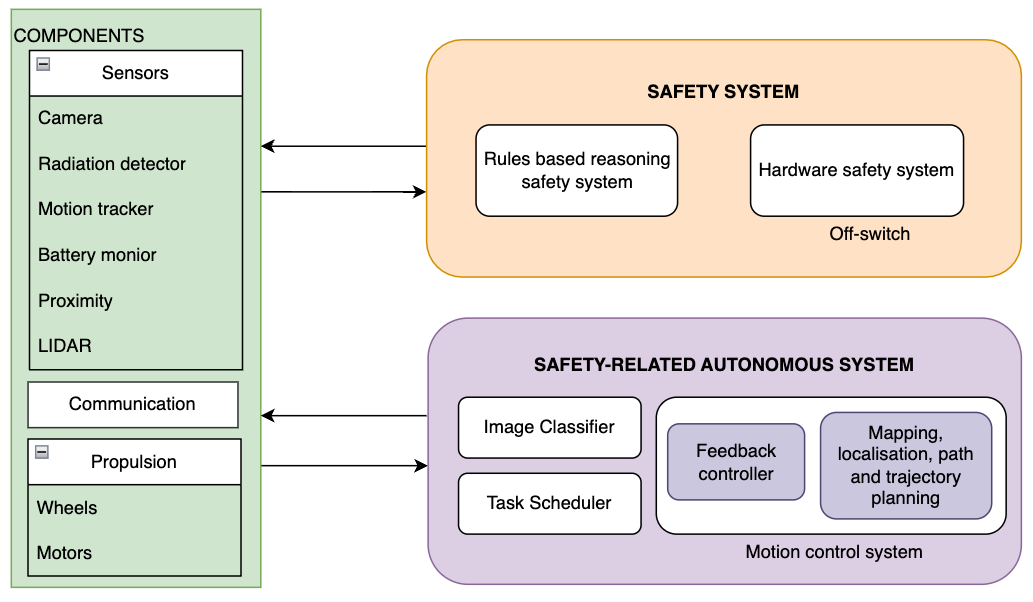
\includegraphics[scale=0.26]{SystArchitecture.png}}
    \caption{Autonomous System Architecture. Components and sub-systems are illustrative examples of types common in RAS.
    }
    \label{Fig:SArchitecture}
\end{figure}


\subsection{From Design to Safety Requirements}
%\marienote{An alternative title: From Design to Safety Requirements}
\label{sec:HazardAnalisys}
Within the proposed approach, the process for defining safety requirements for autonomous robots highly regulated domains takes the steps shown in the Fig~\ref{Fig:Process}:


\begin{enumerate}
    \item[\textbf{Step 1 (Operation Design)}:] outline the objectives and scope of the task to be performed, location and environment. At this stage, there are gathering the requirements for the operation. 
    \item[ \textbf{Step 2 (Hazard  Analysis and Safety Function Definition)}:] identify potential risks and safety concerns associated with the operation and system operation, and identify the safety functions which will mitigate the hazards.
    \item[\textbf{Step 3 (Requirements Identification and Allocation)}:] develop requirements from the hazard analysis and allocate to either the SS (Safety System) or SRAS (Safety-Related Autonomous System).
\end{enumerate}
\textbf{Steps 2} and \textbf{3} are iterated to identify hazards emerging from the design of the system architecture. In \textbf{Step 3}, it is proposed to allocate requirements into three main groups:

\begin{compactitem}
    \item \textbf{\textit{Safety Requirements (SR)}} are allocated to the SIF. These are identified by examining: compliance with \textbf{safety} standards and regulations, hazard analysis and risk assessment, fail-safe mechanisms, emergency shutdown procedures and safety-critical software development practices. 

    \item \textbf{\textit{Standards and Relevant Good Practice Requirements (RGPR)}} relate to adhering to best practice and \textbf{industry} standards, which specify the overall performance and reliability of the system. These may include: engineering and coding standards and guidelines, implementing redundancy, regular maintenance and inspection.

    \item \textbf{\textit{Operational Requirements (OR)}} typically consists of the functional requirements required for the system and are relate to the successful execution of the operation, such as  visiting specific inspection points.
\end{compactitem}

\noindent Each requirement is associated with either the SRAS or SS.

\begin{figure}[t]    
    \centering{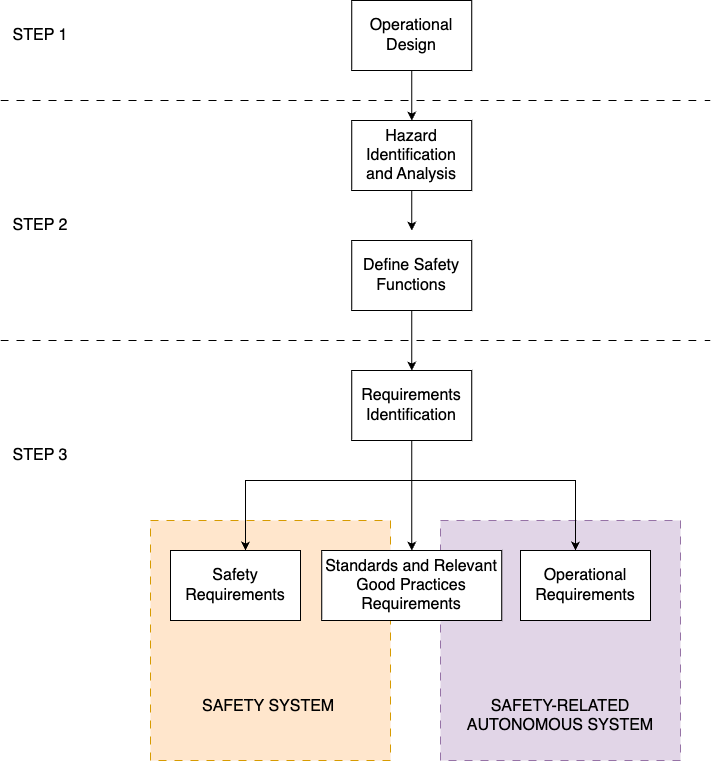
\includegraphics[scale=0.32]{requirements_02.png}}
    \caption{3-step process for defining safety requirements%begins with operational design, followed by hazard analysis and safety function definition. Finally, requirements are identified based on three group and allocated to the appropriate system(s).
    \label{Fig:Process}}
\end{figure}


\section{Results obtained thus far: Case study}
\label{sec:case_study}

The case study is defined as a hypothetical operation involving routine inspections in a nuclear facility; a critical scenario for the operational integrity of nuclear plants. The operation is to perform regular inspections in a space containing radioactive material, with the primary objective being the capture of high-quality images for analysis and assessment. \textbf{Step 1} of the approach shown in Fig.~\ref{Fig:Process} is assumed to have been conducted outside of this case study. Consequently, the challenge lies in identifying the requirements for an autonomous robot to carry out the operation. \medskip%Additional operational assumptions include receiving a detailed inspection point map, positioning the charging station outside the inspection room for accessibility, and assuming stable radiation levels within the inspection room once the robot is deployed. 

%\subsubsection{Hazard identification and analysis}
\noindent\textbf{Step 2 (Hazard Analysis and Safety Function Definition)}:
The \textit{hazard identification} was primarily based on a review of safety reports and open-source papers with similar safety cases~\cite{InspectionRoverCaseStudy,RequirementsRP}. Additionally, published hazard lists and checklists were considered as sources to examine hazard analyses in similar systems~\cite{HazardsCheckList}.

During the \textit{hazard analysis}, each identified hazard is systematically linked to one or more safety functions (\textit{SFs}), which are designed to mitigate or control the associated risks. %This process involves defining safety functions that specifically address the identified hazards, drawing upon a thorough understanding of their potential consequences. 
%For instance, a hazard such as ``collision with physical obstacles'' may be mitigated through the implementation of safety function ``Prevent collision'' (\textbf{SF1}). Similarly, the hazard of ``running out of battery'' (\textbf{H2}) can be addressed by the safety function ``Prevent running out of power'' (\textbf{SF2}). By delineating these safety functions, clear objectives for system design and operation are established, ensuring the safety and integrity of the nuclear facility. 
Through this work four primary \textit{safety functions} have been identified which address the following identified hazards:

\begin{itemize}
    \item [\textbf{SF1}] Prevent collision.
    \item [\textbf{SF2}] Prevent running out of power.
    \item [\textbf{SF3}] Prevent the robot from being exposed to excessively high levels of radiation.
    \item [\textbf{SF 4}] Ensure all reachable inspection points are visited.
\end{itemize}

For reasons of space%\louisenote{I would just say "For reasons  of space"}
, a list of all hazards and their associated safety functions is not presented. \footnote{If accepted, we will include a link to a document containing the full list.}

%We show a subset of the list of the hazards and the Safety Function associated to them are presented on the Table~\ref{tab:requirements}\footnote{If accepted, we will include a link to a document containing the full list.}. 

%\subsubsection{Requirements Identification and Allocation to SRAS and SS}
%\label{sec:req_ident}

\medskip
\noindent\textbf{Step 3 (Requirements Identification and Allocation)}: 
%For the case study, the system architecture detailed in \S\ref{sec:research_approach} is adopted. The core control system forms the SRAS. Tasked with sensor data processing, robot navigation, and executing operations pertinent to capturing images and referencing location/time. The other major component is the Safety System which is responsible for implementing the rules-based SIF.
The requirements identification process involves the following steps: (1) Identifying \textit{parent} mitigation requirements for each safety function 
(2) Breaking down the parent requirements into more specific \textit{children} requirements, thereby establishing a hierarchical structure that facilitates clarity and organisation. This hierarchical approach allows for the extension of the hierarchy as long as children requirements can be identified by their parent. (3) Allocating and assigning requirements to each respective system. An example of this process is presented in  Fig.~\ref{Fig:ReqH}. It's important to emphasise that the identification of hazards and subsequent safety requirements is a systematic process consistently applied throughout the project life-cycle. This approach ensures comprehensive coverage and alignment with safety goals.


\begin{figure}[t] 
    \centering{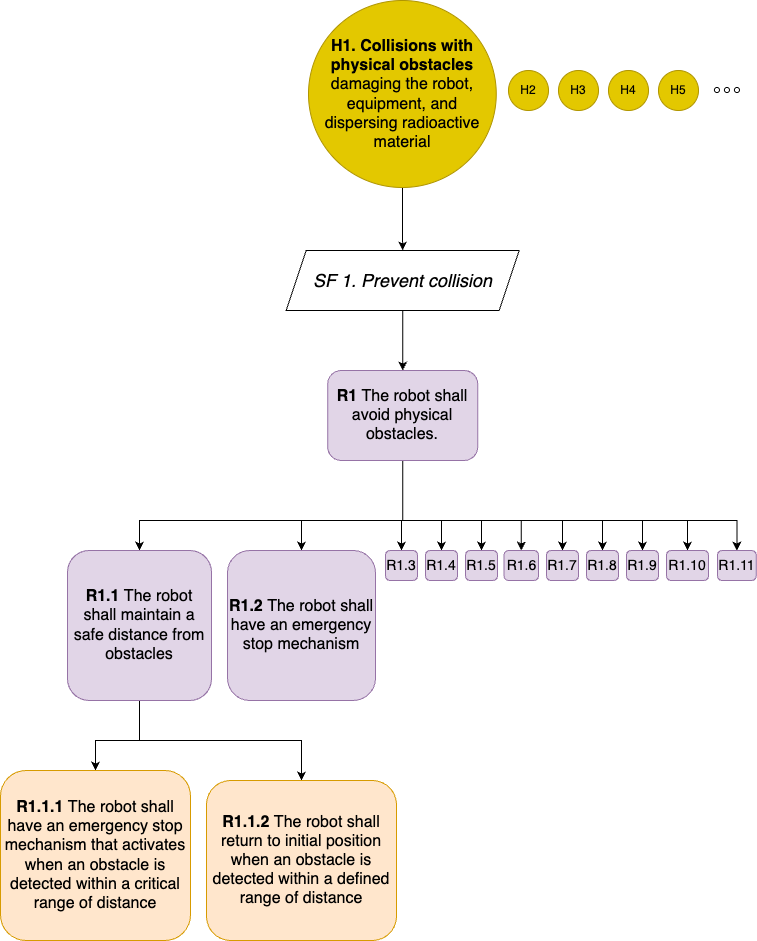
\includegraphics[scale=0.32]{Example.png}
    \caption{Illustrates how the identified hazards are used to identify safety functions with subsequent requirement identification. Requirements are often linked in a hierarchical way as shown above.}
    \label{Fig:ReqH}}
\end{figure}

%Requirements are traceable to the Safety Functions and the hazards which beget them. The terms \emph{parent} and \emph{children} refer to a hierarchical relationship between mitigation requirements. In Fig.~\ref{Fig:ReqH}, \emph{R1} is a parent requirement for all requirements associated with Safety Function 1 (SF 1) which mitigates the  hazard 1 (H1). Notably, \emph{R1.1} functions as a child requirement of \emph{R1}. This child requirement further branches into specific requirements, like \emph{R1.1.1} and \emph{R1.1.2}. This illustrates a concise hierarchical structure where parent requirements guide overarching goals and their children requirements provide detailed strategies for risk mitigation.\louisenote{I feel like a lot of this repeats information in the previous paragraph - can we get the whole parent-child description into one paragraph?}

Requirements are allocated to the respective systems as defined in \S\ref{sec:research_approach}. It is important to highlight that safety system-associated requirements must be incorporated into the logic of the rules-based reasoning system, which comprises the SS. Meanwhile, operational requirements are considered in the SRAS. Standards and relevant good practice are applied for both the SS and SRAS but with differing degrees of rigour.

%As a preliminary result, in Table~\ref{tab:requirements} we present the list of requirements, allocated to either the SS or SRAS. The hazard is explicitly outlined in the ``Source'' column and related to its respective Safety Function, along with requirements identification and allocation.

%In this case study, safety requirements relating to the confirmation of image location ensuring that the captured images correspond to the intended areas, are not currently considered. Although it impacts robot design, this aspect will be included in future analyses, acknowledging its significance for safety in image analysis.

\section{Timeline Planned}

To ensure the timely and organised execution of the research activities, a timeline presented in Fig~\ref{fig:gantt} has been planned for the entire 42-month project duration. This timeline provides an overview of the planned tasks defined in \S \ref{sec:resmethod} -- \ref{sec:plan}, offering insight into the structured progression of the research.
%\marienote{You should say where you are and what has been done exactly somewhere in this section}

Key steps have been completed in the research plan. Initially, the mission and assumptions were defined, followed by thorough hazard identification and analysis. Subsequently, requirements were identified and allocated to the respective systems (SRAS and SIF) in alignment with the proposed system architecture. Moving forward, the next steps involve developing a rules-based reasoning SS to meet specific SIF requirements and integrating this implementation with an SRAS. Alongside implementation and integration, rigorous verification will be conducted using formal methods and testing approaches. Additionally, there will be a demonstration of how the developed SIFs can be verified against properties derived from hazard analyses, ensuring end-to-end traceability from requirements to verified code. Lastly, the proposed architecture and approach will be evaluated using a case study from the UK nuclear industry, while also discussing the limitations of the initial results and potential contributions to the use of autonomous robots in highly regulated domains.

\begin{figure}[t]
  \centering
  \begin{ganttchart}[
    hgrid,
    vgrid,
    x unit=0.15cm,
    y unit title=0.25cm,
    y unit chart=0.25cm,
    title height=1,
    progress label text={},
    bar height=0.5,
    group right shift=0,
    group top shift=.6,
    group height=.3,
    title label font=\tiny,
    bar label font=\tiny,
    group label font=\tiny,
    milestone label font=\tiny,
    today label font=\tiny,
    vrule label font=\tiny
    ]{1}{42} 
    \gantttitle{Timeline (Months)}{42} \\
    \gantttitlelist{1,4,...,42}{3} \\ 
    \ganttbar[progress=100]{Literature review}{1}{5} \\ %elem0
    \ganttbar[progress=100]{Research approach development}{5}{6} \\ %elem1
    \ganttbar[progress=100]{Case study design}{6}{7} \\ %elem2
    \ganttbar[progress=100]{Hazard identification \& analisys}{6}{10} \\ %elem3
    \ganttbar[progress=100]{Req. identification \& allocation}{11}{15} \\ %elem4
    \ganttbar[progress=0]{Implementation rules-based SS}{16}{22} \\ %elem5
    \ganttbar[progress=0]{Verification rules-based SS}{18}{30} \\ %elem6
    \ganttbar[progress=0]{Integration SS with SRAS}{23}{28} \\ %elem7    
    \ganttbar[progress=0]{Deployment rules-based SS}{31}{37} \\ %elem8
    \ganttbar[progress=0]{Project evaluation}{31}{37} \\ %elem9 
    \ganttbar[progress=0]{Report research findings}{38}{42} %elem10
 
    \end{ganttchart}
    \caption{Planned Timeline}
    \label{fig:gantt}
\end{figure}


\section{Conclusion}

In this research, the critical challenge of ensuring the safety of autonomous robots operating in hazardous environments is explored. The high-level research methodology and plan are outlined (\S\ref{sec:resmethod}--\ref{sec:plan}). Subsequently, the approach to defining the requirements for RAS used in highly-regulated domains is presented (\S\ref{sec:research_approach}). This research primarily focuses on presenting a case study (\S\ref{sec:case_study}) within the context of the UK nuclear regulatory regime, where such robots have the potential to play a critical role in enhancing safety, efficiency, and data collection within hazardous operations. The main anticipated contribution of this research is an approach for defining safety requirements for autonomous robots operating in hazardous environments, aligning with the principles and methodologies of RE. This will help to facilitate the provision of reliable, autonomous robots that can safely be used in critical domains. %\marienote{added the last sentence, might be a bit of a stretch but I thought the conclusion should be a bit stronger}


\begin{thebibliography}{00}

\bibitem{SIFinHighDemandMode} Bukowski, J. V., \& Goble, W. M. (2017, January). Properly crediting diagnostics in safety instrumented functions for high demand processes. In 2017 Annual Reliability and Maintainability Symposium (RAMS) (pp. 1-6). IEEE.
\bibitem{FunctionalSafety} International Electrotechnical Commission. (2000). Functional safety of electrical/electronic/programmable electronic safety related systems. IEC 61508.
\bibitem{NS-TAST-GD-005} Office for Nuclear Regulation (ONR). Guidance on the demonstration of ALARP (as low as reasonably practicable). Nuclear Safety Technical Assessment Guide NS-TAST-GD-005.
\bibitem{RERegulatoryCompliance} Kempe, E., \& Massey, A. (2021, September). Perspectives on regulatory compliance in software engineering. In 2021 IEEE 29th International Requirements Engineering Conference (RE) (pp. 46-57). IEEE.
\bibitem{RE4AI}Ahmad, K., Bano, M., Abdelrazek, M., Arora, C., \& Grundy, J. (2021, September). What’s up with requirements engineering for artificial intelligence systems?. In 2021 IEEE 29th International Requirements Engineering Conference (RE) (pp. 1-12). IEEE.
\bibitem{REChallenges} H. Belani, M. Vukovic, and Z. Car, “Requirements engineering challenges in building AI-based complex systems,” in 2019 IEEE 27th International Requirements Engineering Conference Workshops (REW). IEEE, 2019, pp. 252–255. 
\bibitem{Louise&Chris} Anderson, C. R., \& Dennis, L. A. (2023). Autonomous Systems' Safety Cases for use in UK Nuclear Environments. arXiv preprint arXiv:2310.02344. Online resource. https://doi.org/10.48420/19512010, 2022.
\bibitem{PintoA} Pinto, A. (2021, December). Requirement specification, analysis and verification for autonomous systems. In 2021 58th ACM/IEEE Design Automation Conference (DAC) (pp. 1315-1318). IEEE.
\bibitem{RBSystemUAV} Hu, J., Wang, T., Zhang, H., Pan, Q., Zhang, J., \& Xu, Z. (2023). A review of rule-based collision avoidance technology for autonomous UAV. Science China Technological Sciences, 66(9), 2481-2499. 
\bibitem{FormalSpecificationAndVerification} Luckcuck, M., Farrell, M., Dennis, L. A., Dixon, C., \& Fisher, M. (2019). Formal specification and verification of autonomous robotic systems: A survey. ACM Computing Surveys (CSUR), 52(5), 1-41.
\bibitem{farrell2018robotics} Farrell, M., Luckcuck, M., \& Fisher, M. (2018). Robotics and integrated formal methods: Necessity meets opportunity. In Integrated Formal Methods. (pp. 161-171). Springer.
\bibitem{MCAPL}Dennis, L. A. (2018). The MCAPL framework including the agent infrastructure layer and agent java pathfinder. The Journal of Open Source Software.
\bibitem{Do-178c} Moy, Y., Ledinot, E., Delseny, H., Wiels, V., \& Monate, B. (2013). Testing or formal verification: Do-178c alternatives and industrial experience. IEEE software, 30(3), 50-57.
\bibitem{InspectionRoverCaseStudy} Bourbouh, H., Farrell, M., Mavridou, A., Sljivo, I., Brat, G., Dennis, L. A., \& Fisher, M. (2021, May). Integrating formal verification and assurance: an inspection rover case study. In NASA Formal Methods Symposium (pp. 53-71). Cham: Springer International Publishing.
\bibitem{RequirementsRP} Farrell, M., Mavridou, A., \& Schumann, J. (2023, April). Exploring Requirements for Software that Learns: A Research Preview. In International Working Conference on Requirements Engineering: Foundation for Software Quality (pp. 179-188). Cham: Springer Nature Switzerland.
\bibitem{HazardsCheckList} NASA (1987). Methodology for the conduct of NSTS hazard analysis. National Space Transportation System, NSTS 22254 edition.


\end{thebibliography}

\end{document}
